
\chapter{Einleitung}

Elektrizität ist in unserem Alltag allgegenwärtig. Sie findet Anwendung in Handys,
Computer, Haushaltsgeräte, Autos, Züge und Flugzeuge, um einige Beispiele zu nennen.
Elektrizität ist eine der wichtigsten Energieformen, die wir nutzen.

Neben der technischen Anwendung hat die Elektrizitätslehre auch eine grosse
Bedeutung in der Physik und ist zentral für das grundlegende Naturverständnis.
Die elektromagnetische Kraft ist eine der vier Grundkräfte der Physik.
Das Atom besteht aus einem elektrisch positiv geladenen Atomkern und
elektrisch negativ geladenen Elektronen, die den Atomkern umkreisen.

Dieses Dossier gibt dir eine Einführung in die Elektrizitätslehre.
Dabei wird nicht nur das theoretische Wissen vermittelt, sondern auch
praktische Experimente durchgeführt. Das Dossier enthält die folgenden
Abschnitte:

Im ersten Teil werden die Komponenten eines Stromkreises vorgestellt.
Der Unterschied zwischen Serie- und Parallelschaltung wird erklärt. Im zweiten
Teil werden die Grössen Stromstärke und Spannung eingeführt und erklärt,
wie sie gemessen werden können. Im dritten Teil wird auf die elektrische
Leistung und den elektrischen Widerstand eingegangen. In diesem Zusammenhang
wird das Ohm'sche Gesetz vorgestellt.


\vspace{1cm}

\begin{redbox}
Es ist wichtig, nur die vorgesehenen Bauteile zu verwenden und
nur die gezeigten Schaltungen aufzubauen. Bei unsachgemässer Verwendung
kann es zu Kurzschlüssen und Beschädigungen kommen.
\end{redbox}



\newpage
\section{Bauteile des Experimentierkastens}

Der Experimentierkasten enthält verschiedene Bauteile, siehe
\fref{fig:components}. Es gibt zwei Batteriehalter, zwei Schalter und
zwei Lampenhalter. Weiter sind zwei Messgeräte, ein Amperemeter und ein Voltmeter vorhanden.
Es gibt vier feste Widerstände und einen variablen Widerstand. Verbunden werden kann
alles mit Kabeln.



\begin{figure}[h!]
    \centering
    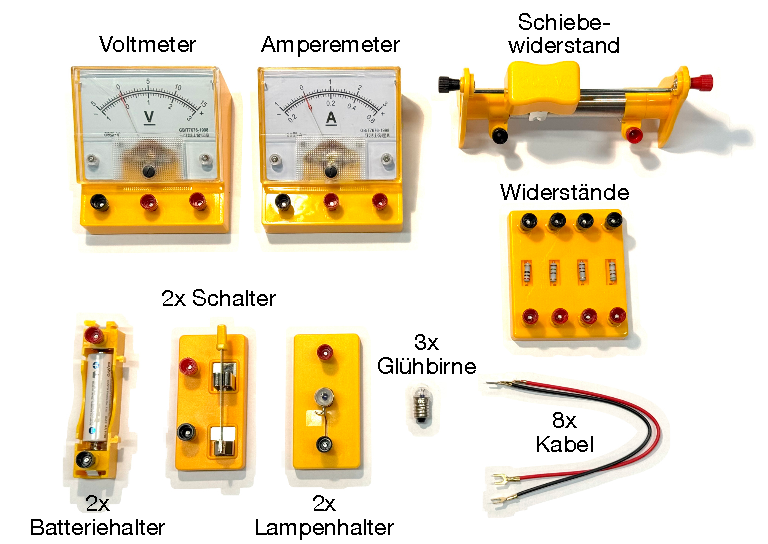
\includegraphics[width=12cm]{_images/bauteile.pdf}
    \caption{Bauteilübersicht}
    \label{fig:components}
\end{figure}


\section{Kabel anschliessen}

Die einzelnen Bauteile des Stromkreises können mit den Kabeln verbunden werden.
Dazu muss die Schraube im Gegenuhrzeigersinn gedreht werden. Anschliessend kann
das Kabel mit dem U-förmigen Anschluss verbunden werden. Die Schraube wird
wieder im Uhrzeigersinn gedreht, um das Kabel zu fixieren, siehe \fref{fig:connecting_wires}.

\begin{figure}[h!]
    \centering
    \begin{tikzpicture}
        \node[anchor=north west] at (0,0) {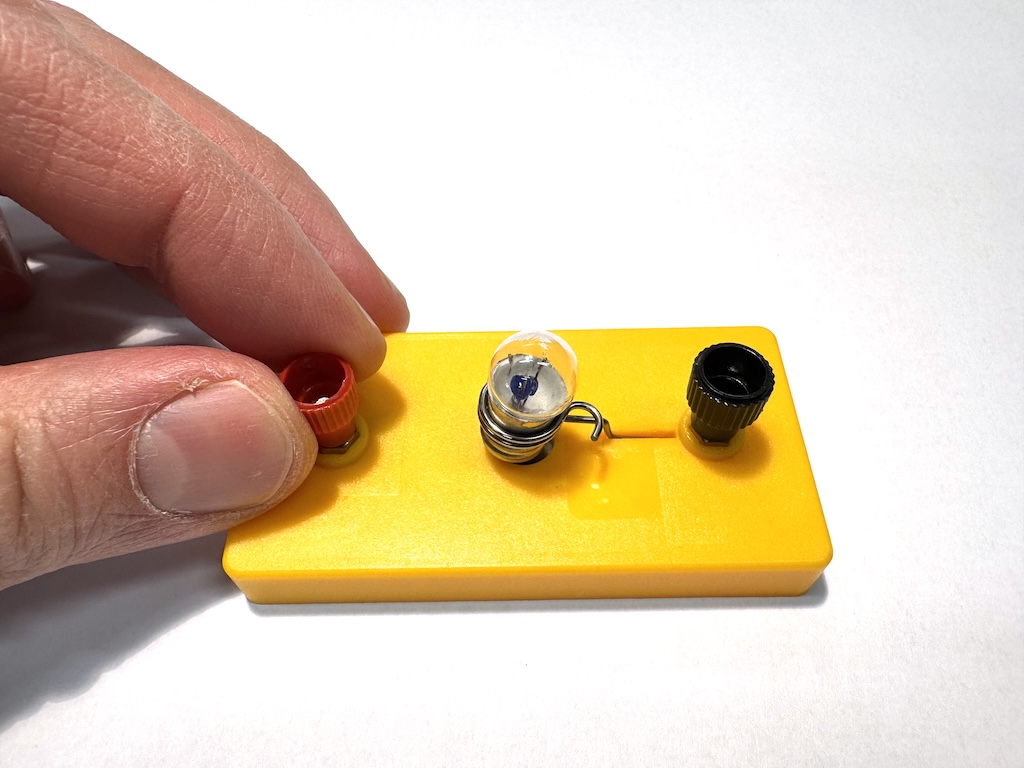
\includegraphics[width=4cm]{_images/kabel_anschliessen_1}};

        \node[anchor=north west] at (6,0) {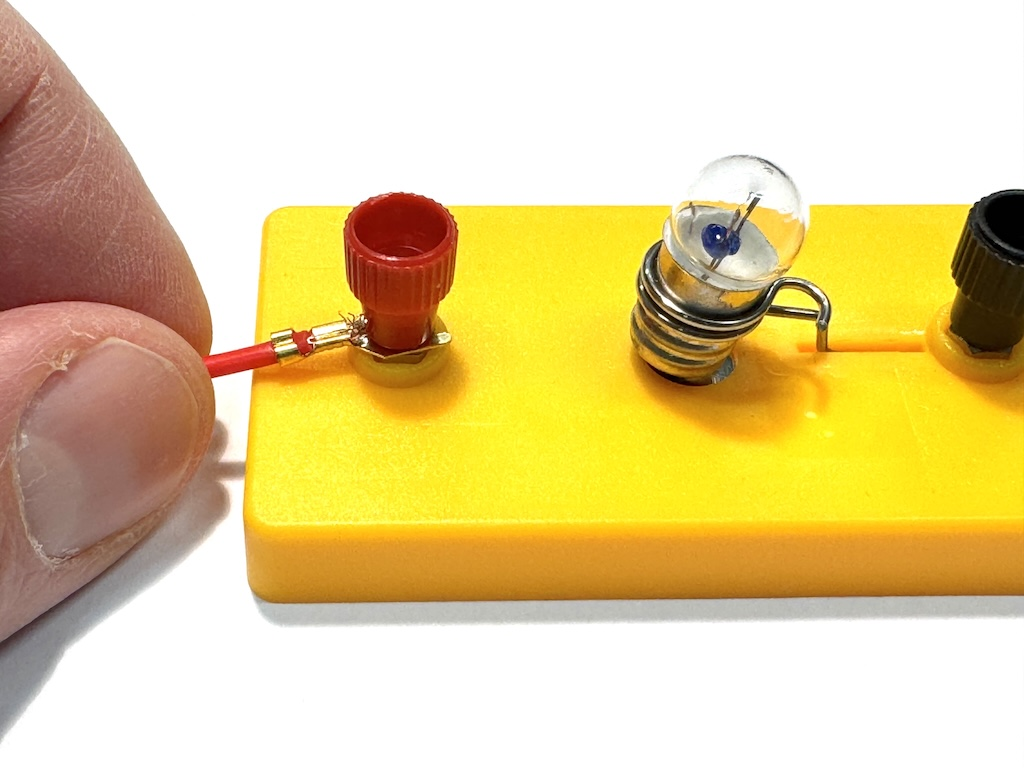
\includegraphics[width=4cm]{_images/kabel_anschliessen_2}};

        \node[anchor=north west] at (11,0) {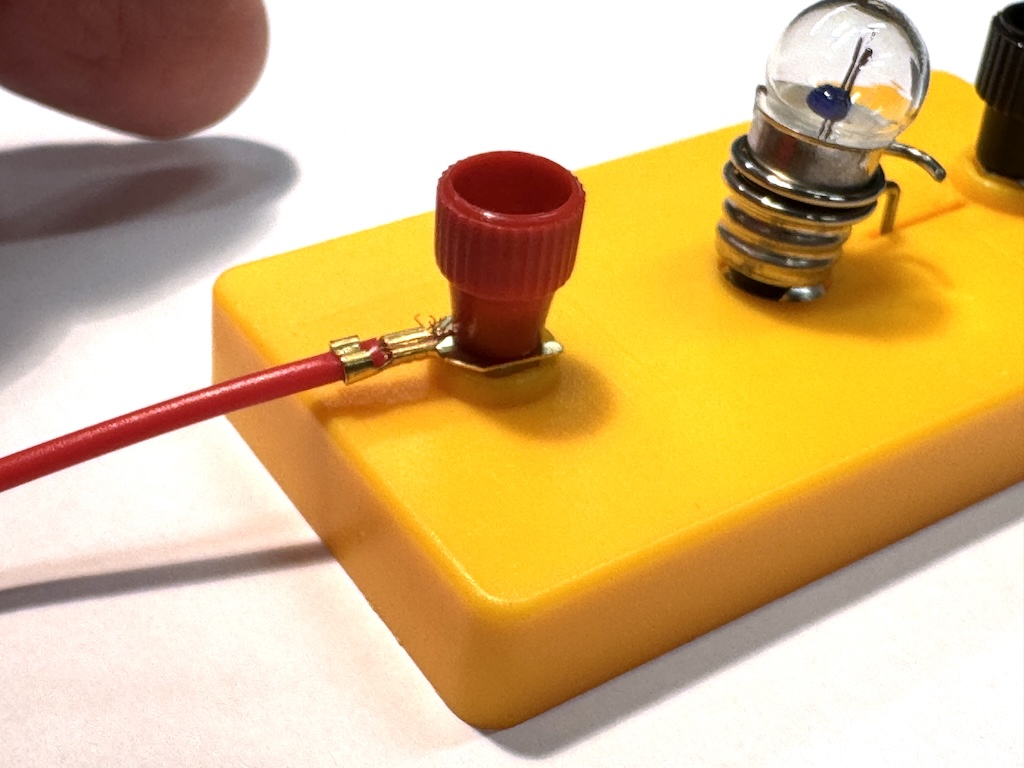
\includegraphics[width=4cm]{_images/kabel_anschliessen_3}};

        \node[anchor=south west] at (0,0) {1.};

        \node[anchor=south west] at (6,0) {2.};

        \node[anchor=south west] at (11,0) {3.};

    \end{tikzpicture}

    \caption{Kabel anschliessen}
    \label{fig:connecting_wires}
\end{figure}


\newpage
\section{Batterie}

Die Batterie muss korrekt in die Halterung eingesetzt werden.
Der Pluspol der Batterie muss bei dem roten Anschluss und der Minuspol
bei dem schwarzen Anschluss zu liegen kommen, siehe \fref{fig:batteryholder}.
Die Feder im Batteriehalter muss immer den Minuspol der Batterie berühren.

\begin{figure}[h!]
    \centering
    \begin{tikzpicture}
        \node[anchor=north west] at (0,0) {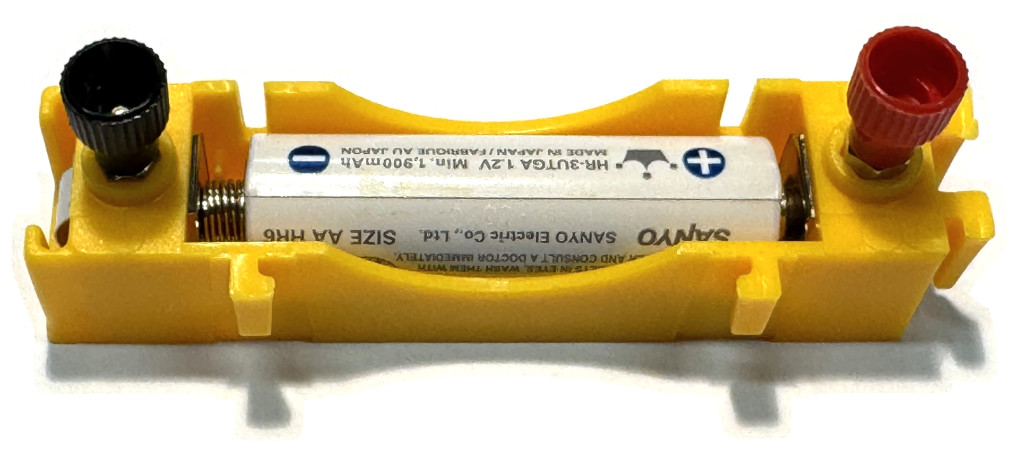
\includegraphics[width=6cm]{_images/batterie_solo}};

        \node[anchor=east] at (0.25,-0.75) {Minuspol (--)};

        \node[anchor=west] at (6.25,-0.75) {(+) Pluspol};

    \end{tikzpicture}

    \caption{Batteriehalter}
    \label{fig:batteryholder}
\end{figure}

Die Batteriehalter sind so konstruiert, dass sie in Serie oder parallel
zusammen geschaltet werden können, siehe \fref{fig:batteryholder_serial} und \fref{fig:batteryholder_parallel}.

\begin{figure}[h!]
    \centering
    \begin{subfigure}[b]{0.4\textwidth}
    \centering
    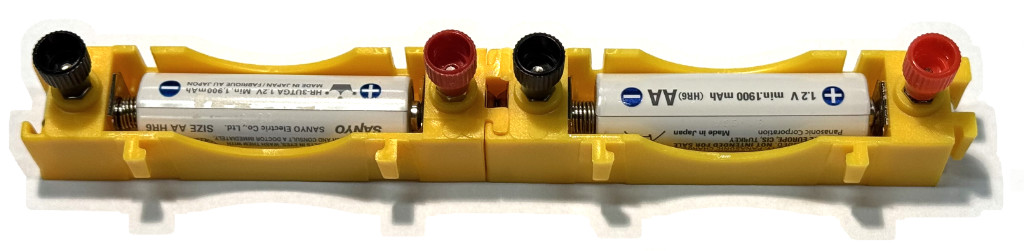
\includegraphics[width=7cm]{_images/batterie_seriell}
    \caption{\label{fig:batteryholder_serial}}
    \end{subfigure}
    \quad
    \begin{subfigure}[b]{0.4\textwidth}
    \centering
    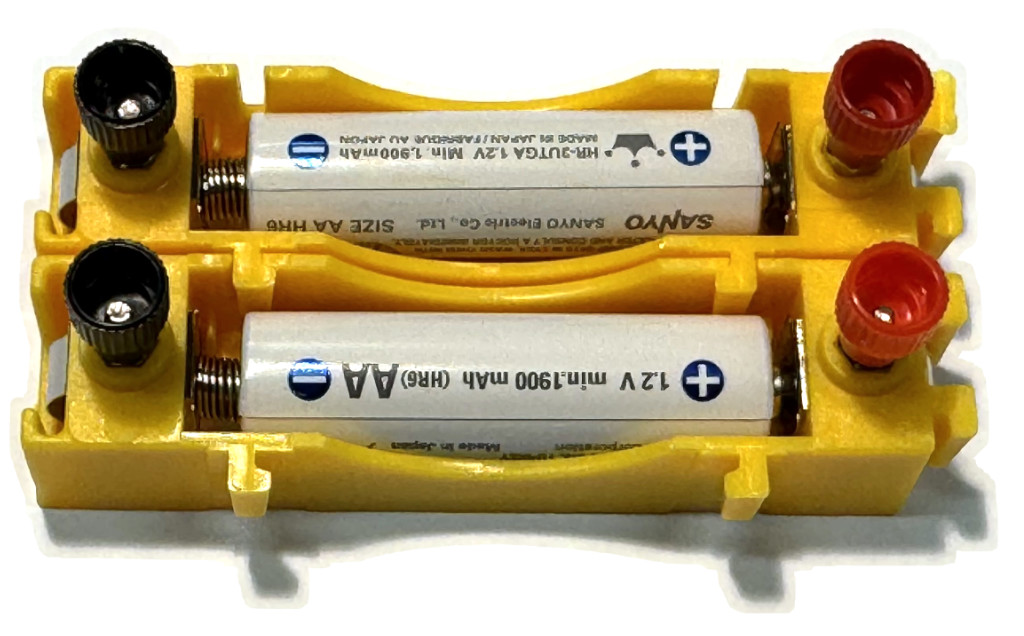
\includegraphics[width=3.8cm]{_images/batterie_parallel}
    \caption{\label{fig:batteryholder_parallel}}
    \end{subfigure}

    \caption{Serienschaltung (a) und Parallelschaltung (b) von Batterien}
\end{figure}


\section{Schaltsymbole}

In der Elektrizität werden Schaltsymbole verwendet, um die Teile des
Stromkreises darzustellen. Hier ist eine Übersicht über einige Schaltsymbole,
welche in diesem Dossier vorkommen.

\begin{figure}[h!]
    \centering
    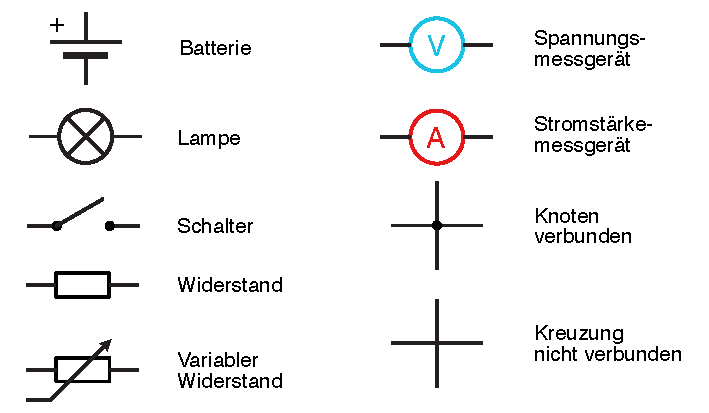
\includegraphics[width=10cm]{_images/schaltsymbole.pdf}
    \caption{Übersicht über alle Schaltsymbole}
    \label{fig:symbols}
\end{figure}
